\documentclass[conference]{IEEEtran}
\usepackage{amsmath}
\usepackage{newtxtext,newtxmath}
\usepackage{graphicx}
\usepackage{booktabs}
\usepackage{xcolor}
\usepackage[hidelinks]{hyperref}
\graphicspath{{../../../results/02-tgape/}}

% Every number in this file comes from results/02-tgape/t1_topology_mapping/summary.md (rule E5).
% All of them are scenario values: synthetic workloads + analytic leaf-spine model (rule E1).

\newcommand{\todo}[1]{\textcolor{red}{[TODO: #1]}}

\begin{document}

\title{T-GAPE: Does the Leaf Level Matter?\\Topology-Aware Rank Mapping for ML Traffic\\on Oversubscribed Leaf-Spine Clusters}

\author{
\IEEEauthorblockN{Divyansh Verma, Aniruddha Badhani, Ashutosh Singh}
\IEEEauthorblockA{Dept.\ of Computer Science and Engineering,
Noida Institute of Engineering and Technology, Greater Noida, India\\
\{0241cs202, 0241cs161, 0241cs203\}@niet.co.in}
}

\maketitle

\begin{abstract}
Communication-aware placement usually stops at the host: it decides which ranks share a machine
and leaves the mapping of hosts onto switches to chance. We ask how much the next level, which
hosts share a leaf switch, matters for modern training traffic, and under what spine
oversubscription. Using a two-tier leaf-spine model, three workloads (MoE with routing affinity,
Megatron with mismatched rank order, and a 3D stencil) and four mapping strategies, we find
that the leaf level adds nothing at 1:1 oversubscription, even though leaf-aware mapping cuts
cross-leaf bytes from 0.55 to 0.31 of traffic for MoE. It matters once the host-only mapping
becomes uplink-bound: at 4:1, hierarchical mapping reaches $0.40\times$ block placement's modelled
communication time for MoE against $0.74\times$ for host-only mapping, and $0.07\times$ against
$0.14\times$ for Megatron. Under NCCL-style ring re-derivation the gaps shrink but hold
($0.42\times$ vs.\ $0.67\times$; $0.11\times$ vs.\ $0.18\times$). For the stencil, bottom-up
mapping is $1.02\times$ block while top-down reaches $0.79\times$: minimising total cut does not
minimise the busiest uplink. All results are scenario values from an analytic model.
\end{abstract}

\begin{IEEEkeywords}
topology mapping, leaf-spine, oversubscription, process placement, distributed training
\end{IEEEkeywords}

% ---------------------------------------------------------------------------------------------
\section{Introduction}

Hierarchical topology mapping is well studied for HPC: Hoefler and Snir compare generic mapping
strategies~\cite{hoefler2011generic}, TreeMatch maps onto machine trees~\cite{jeannot2014treematch},
and Scotch recursively bipartitions process and architecture graphs
together~\cite{pellegrini1996scotch}; see~\cite{hoefler2014overview} for a survey. We do not claim
that two-level mapping is new. The open question is quantitative: \emph{for the traffic of modern
training jobs, how much does mapping hosts onto leaf switches add to host-level placement, and
when?} The answer decides whether a placement tool for GPU clusters needs a topology model at all.

Our companion paper~\cite{cage2026} (CAGE) shows that host-level placement beats block placement
only when the communication graph has significant structure that disagrees with rank order. This
paper takes those cases, adds a leaf-spine fabric, and measures the increment. Our contributions:
\begin{enumerate}
\item A leaf-spine extension of the CAGE cost model with four mapping strategies, evaluated in both
      the rank-pinned and the NCCL ring re-derivation regimes (Section~\ref{sec:model}).
\item Evidence that the leaf level matters exactly when host-only mapping is uplink-bound: never at
      1:1, for some workloads at 2:1, and strongly at 4:1 (Section~\ref{sec:results}).
\item A counter-example in which bottom-up mapping is worse than block placement, traced to a
      mismatch between the min-cut objective and the bottleneck-link cost.
\end{enumerate}

% ---------------------------------------------------------------------------------------------
\section{Background}

GPU clusters are commonly built as folded-Clos (fat-tree) fabrics~\cite{leiserson1985fattrees,
alfares2008fattree}. Each host's NIC connects to a leaf switch; leaves connect to spines. Operators
often provision less uplink bandwidth than the sum of host links, a ratio called
oversubscription~\cite{greenberg2009vl2}. Traffic between hosts on one leaf never touches the
uplinks; traffic between leaves does, spread over spines by ECMP~\cite{rfc2992}. TopoOpt
co-optimises topology and parallelisation for ML jobs~\cite{wang2023topoopt}; FasterMoE uses
topology in MoE expert placement~\cite{he2022fastermoe}. We take the fabric as given and change
only where ranks run.

% ---------------------------------------------------------------------------------------------
\section{Model and Strategies}\label{sec:model}

\textbf{Fabric.} $\Lambda$ leaves, $k=4$ hosts per leaf, $g=8$ GPUs per host. Each host has one NIC
of $B_{\mathrm{nic}}=50$\,GB/s per direction; GPUs in a host share $B_{\mathrm{intra}}=300$\,GB/s.
Each leaf has one aggregated uplink of $B_{\mathrm{up}} = kB_{\mathrm{nic}}/\rho$ for
oversubscription $\rho\in\{1,2,4\}$. The spine is an ideal non-blocking crossbar (perfect ECMP).

\textbf{Cost.} Given the rank traffic matrix $M$, the host placement and the leaf of each host,
let $N_h$ be host $h$'s larger direction of cross-host bytes, $U_\ell$ leaf $\ell$'s larger direction
of cross-leaf bytes, and $X_h$ host $h$'s intra-host bytes. The modelled per-step communication time is
\begin{equation}
T = \max\Big(\max_h \tfrac{N_h}{B_{\mathrm{nic}}},\ \max_\ell \tfrac{U_\ell}{B_{\mathrm{up}}}\Big)
    + \max_h \tfrac{X_h}{B_{\mathrm{intra}}}.
\end{equation}
A mapping is \emph{uplink-bound} when its busiest uplink time exceeds its busiest NIC time. Like
CAGE's host model, $T$ ranks mappings; it does not predict seconds.

\textbf{Strategies.} All use CAGE's exact-capacity partitioner (METIS, capacity repair, pairwise
swap refinement, best of three seeds):
\begin{itemize}
\item \emph{block}: ranks in order onto hosts, hosts in order onto leaves (launcher default);
\item \emph{flat}: CAGE host partition with host labels matched to block placement, hosts onto
      leaves in that order (host-aware, leaf-oblivious);
\item \emph{hierarchical} (bottom-up): CAGE host partition, then partition the host traffic graph
      onto leaves;
\item \emph{top-down}: partition ranks onto leaves ($kg=32$ slots each), then onto hosts within each leaf.
\end{itemize}

\textbf{Regimes.} In the \emph{pinned/fixed} regime the traffic matrix moves with the ranks.
In the \emph{NCCL} regime each recorded collective is re-expanded for every candidate as a ring
ordered by leaf and then by host, as NCCL derives rings from the topology; each strategy takes the
better of two partitioning objectives (all traffic in rank order, or rank-pinned traffic plus a
clique expansion of the collectives), as in CAGE.

\textbf{Workloads} (128 ranks, 16 hosts, 4 leaves). These are the cases where host placement
pays~\cite{cage2026}: (i) \emph{MoE}, 128-way expert parallelism, top-2, Zipf 1.0 popularity, data
groups interleaved across ranks with routing affinity 0.6, plus a dense 2\,GB allreduce (dropped in
the pinned regime, re-ringed in the NCCL regime); (ii) \emph{Megatron} TP 8, PP 4, DP 4 with
randomly relabelled ranks; (iii) a \emph{3D stencil} on an $8\times4\times4$ grid with 4\,MB halos,
which is all point-to-point, so both regimes coincide.

% ---------------------------------------------------------------------------------------------
\section{Results}\label{sec:results}

Fig.~\ref{fig:t1} plots modelled time relative to block for every workload and strategy;
Table~\ref{tab:t1} lists the key rows.

\begin{figure*}[t]
\centering
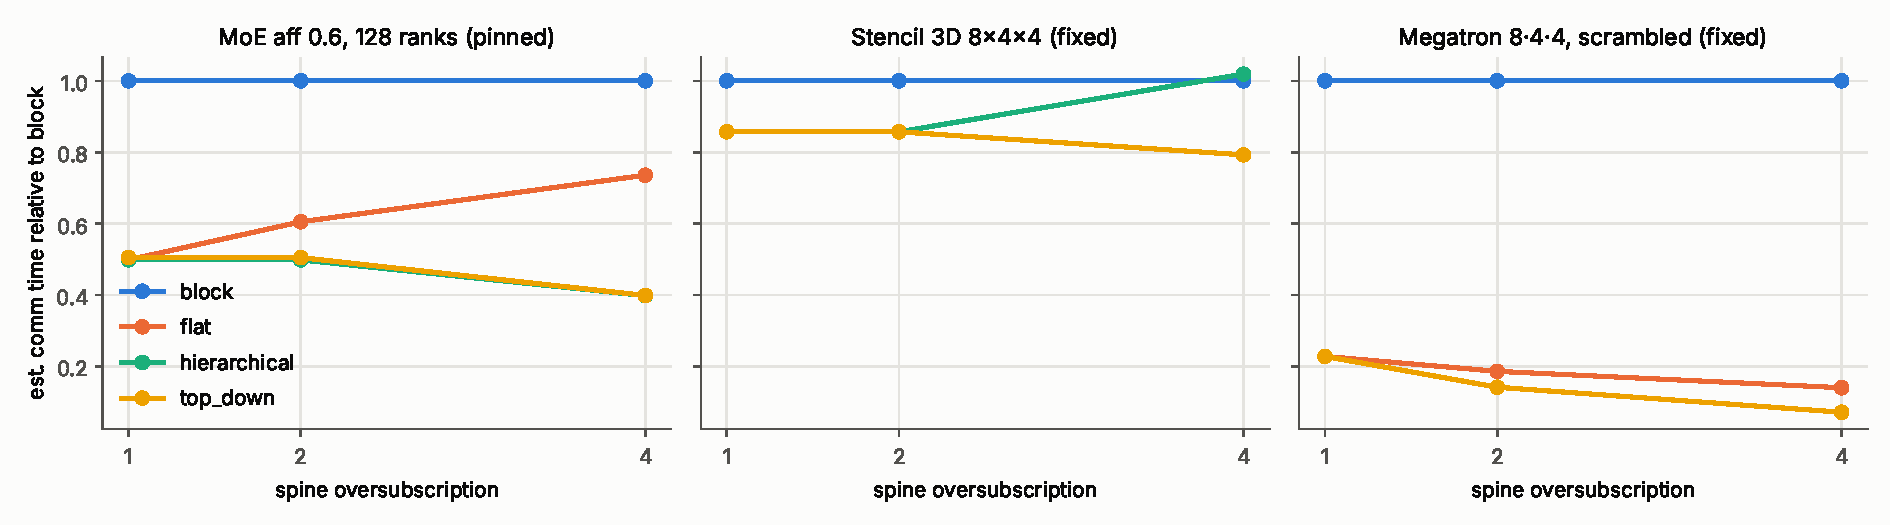
\includegraphics[width=\textwidth]{t1_topology_mapping/time_vs_oversubscription.pdf}
\caption{T1: modelled communication time relative to block placement against spine
oversubscription, per workload and regime. Scenario values.}\label{fig:t1}
\end{figure*}

\begin{table}[t]
\caption{Modelled time relative to block, and whether the mapping is uplink-bound (U). Last column: share of traffic crossing leaves, flat $\to$ hierarchical (T1).}\label{tab:t1}
\centering\footnotesize
\setlength{\tabcolsep}{3pt}
\begin{tabular}{@{}llrrrr@{}}
\toprule
Workload & $\rho$ & flat & hierarchical & top-down & cross-leaf \\
\midrule
MoE, pinned   & 1 & 0.498   & 0.498   & 0.504   & $0.546\to0.313$ \\
              & 2 & 0.605 U & 0.498   & 0.504   & \\
              & 4 & 0.736 U & 0.398 U & 0.398 U & \\
MoE, NCCL     & 1 & 0.525   & 0.525   & 0.531   & $0.379\to0.221$ \\
              & 4 & 0.674 U & 0.419 U & 0.419 U & \\
Megatron, fixed & 1 & 0.228 & 0.228   & 0.228   & $0.058\to0.003$ \\
              & 4 & 0.140 U & 0.071   & 0.071   & \\
Megatron, NCCL & 1 & 0.219  & 0.219   & 0.219   & $0.048\to0.003$ \\
              & 4 & 0.182 U & 0.109   & 0.109   & \\
Stencil 3D    & 1 & 0.857   & 0.857   & 0.857   & $0.158\to0.158$ \\
              & 4 & 1.019 U & 1.019 U & 0.792 U & \\
\bottomrule
\end{tabular}
\end{table}

\subsection{At 1:1 the leaf level adds nothing}
At $\rho=1$, flat and hierarchical mapping give the same modelled time for every workload (MoE
pinned 0.498, Megatron 0.228, stencil 0.857), although hierarchical mapping cuts the share of
traffic crossing leaves from 0.546 to 0.313 for MoE and from 0.058 to 0.003 for Megatron. No
mapping is uplink-bound: the busiest NIC is the bottleneck, and the NIC load depends only on the
host partition. Cross-leaf bytes, the metric topology-mapping papers often report, are the wrong
target when the uplinks are not the bottleneck.

\subsection{Under oversubscription it is decisive}
At $\rho=2$, flat MoE mapping becomes uplink-bound (busiest uplink 1728\,ms vs.\ busiest NIC
1402\,ms) and rises to $0.605\times$ block, while hierarchical mapping stays NIC-bound at
$0.498\times$. At $\rho=4$ the gap widens: $0.398\times$ vs.\ $0.736\times$ for MoE and $0.071\times$
vs.\ $0.140\times$ for Megatron. Hierarchical Megatron mapping never becomes uplink-bound: its
busiest uplink carries 86\,ms against a 408\,ms NIC. With the leaf level, Megatron's time is the
same at every oversubscription (1.21\,s per step); without it, the flat mapping's time grows from
1.21\,s to 2.38\,s. The rule is simple and can be checked before anything moves: \emph{map onto
leaves when the host-only mapping is uplink-bound}.

\subsection{NCCL re-ringing narrows but keeps the gap}
In the NCCL regime the dense MoE allreduce and Megatron's TP and DP rings are rebuilt for each
mapping in leaf-then-host order, which removes part of the cross-leaf ring traffic even for
leaf-oblivious mappings. At $\rho=4$ the gap shrinks from $0.398$ vs.\ $0.736$ to $0.419$ vs.\
$0.674$ for MoE, and from $0.071$ vs.\ $0.140$ to $0.109$ vs.\ $0.182$ for Megatron. The ratio of
flat to hierarchical time falls from 1.97 to 1.67 for Megatron, but leaf-aware mapping still wins
by a wide margin. Leaving the ring order to the library is not a substitute for placing hosts.

\subsection{Min-cut is not min-max: the stencil}
For the 3D stencil at $\rho=4$, flat and hierarchical mapping are \emph{worse} than block
($1.019\times$), while top-down reaches $0.792\times$. All four strategies send the same share of
traffic across leaves (0.158). What differs is how evenly it is spread: block, flat and hierarchical
leave the busiest uplink at 2.56\,ms, whereas top-down balances it to 1.92\,ms. Bottom-up mapping
fixes host shapes that minimise the host cut and then cannot arrange them onto leaves any better
than block order does; the slight loss comes from the larger intra-host term of the partitioned
hosts. The partitioners minimise \emph{total} cut while the fabric is limited by its \emph{busiest}
link. On the ML workloads top-down and hierarchical agree (MoE 0.398 and 0.398, Megatron 0.071 and
0.071), so for them a two-level greedy mapping suffices; for regular HPC grids the choice matters.

% ---------------------------------------------------------------------------------------------
\section{Threats to Validity}

\textbf{Synthetic inputs.} All workloads are models, chosen from the cases where host placement
pays. Where host placement does not pay (data parallelism, Megatron in launcher order), we have not
tested whether leaf placement does.
\textbf{Fabric model.} One aggregated uplink per leaf with ideal ECMP hides flow collisions on
individual spine links, which in practice make oversubscription worse. Three-tier fat-trees,
rail-optimised fabrics with one NIC per GPU, and dragonflies~\cite{kim2008dragonfly} are not modelled.
\textbf{Single configuration.} Only 4 hosts per leaf, 16 hosts and 128 ranks were run.
\textbf{Cost model.} Bandwidth only; no latency, compute overlap or dependencies. Times rank
mappings; they do not predict seconds.
\textbf{Validation path.} A flow- or packet-level simulator such as ASTRA-sim's network
backend~\cite{rashidi2020astra} or SimGrid~\cite{casanova2014simgrid}, and eventually a real
cluster, should replay these mappings.

% ---------------------------------------------------------------------------------------------
\section{Conclusion}
For modern training traffic on leaf-spine clusters, the leaf level is irrelevant at 1:1
oversubscription and decisive at 4:1, and the switch between the two is visible in the model: it
happens when the host-only mapping becomes uplink-bound. NCCL's ring re-derivation narrows the gap
but does not close it. Bottom-up two-level mapping can lose to block placement on regular grids
because it minimises total cut rather than the busiest link; a min-max objective at the leaf level
is the natural fix and the next experiment.

\section*{Artifact Availability}
Code, the T1 script and its results are available at \url{https://github.com/n0tdivyansh/cage-research};
\texttt{cage run --paper 2} regenerates them.

\bibliographystyle{IEEEtran}
\bibliography{../../01-cage/draft/refs}

\end{document}
